\section{Page Classifier}\label{sec:page_classifier}

The page classifier module is responsible for classifying the crawled pages into product pages and non-product pages - which is essentially a binary classification problem.
This module is crucial for filtering out irrelevant pages and ensuring that only product pages are processed by the information extractor and product matching modules.
The page classifier is able to accurately identify product pages by analyzing the content and structure of the minimized HTML pages.

This takes place in three phases.
\begin{enumerate}
    \item \textbf{Training phase:} In this phase, the page classifier is trained using the labelled dataset of HTML pages.
    The labelled dataset is created using the data annotation application.
    The training phase involves model selection, and model training and fine-tuning.
    \item \textbf{Model evaluation and selection:} In this phase, the trained models are evaluated using a separate validation dataset, and the best performing model is selected for deployment.
    Other factors such as training/inference speed and cost are also considered when selecting the best model.
    \item \textbf{Inference phase:} In this phase, the trained page classifier is used to classify new crawled pages into product pages and non-product pages.
\end{enumerate}

\subsection{Training Phase}\label{subsec:page_classifier_training_phase}

Since the data is unstructured and the HTML pages can vary significantly in terms of content and structure, a deep learning approach is used for the page classification task.
For this purpose, three different model architectures were trained and evaluated.

\begin{itemize}
    \item \textbf{TF-IDF with traditional machine learning classifiers:} This approach involves extracting TF-IDF features from the HTML content and using traditional machine learning classifiers, such as logistic regression, support vector machines (SVM), and random forests, to classify the pages.
    \item \textbf{BERT embeddings with a neural network classifier:} This approach involves using a pre-trained BERT model to generate embeddings for the textual content of the page, which are then fed into a neural network classifier for classification.
    \item \textbf{MarkupLM for document classification:} This approach involves using a pre-trained MarkupLM model, which is specifically designed for processing HTML documents, to classify the pages.
\end{itemize}

In each of the above approaches, the model's hyperparameters were tuned using a grid search approach available in AWS SageMaker, which is illustrated in Figure~\ref{fig:page_classifier_training_phase}.

\begin{figure}[h]
    \centering
    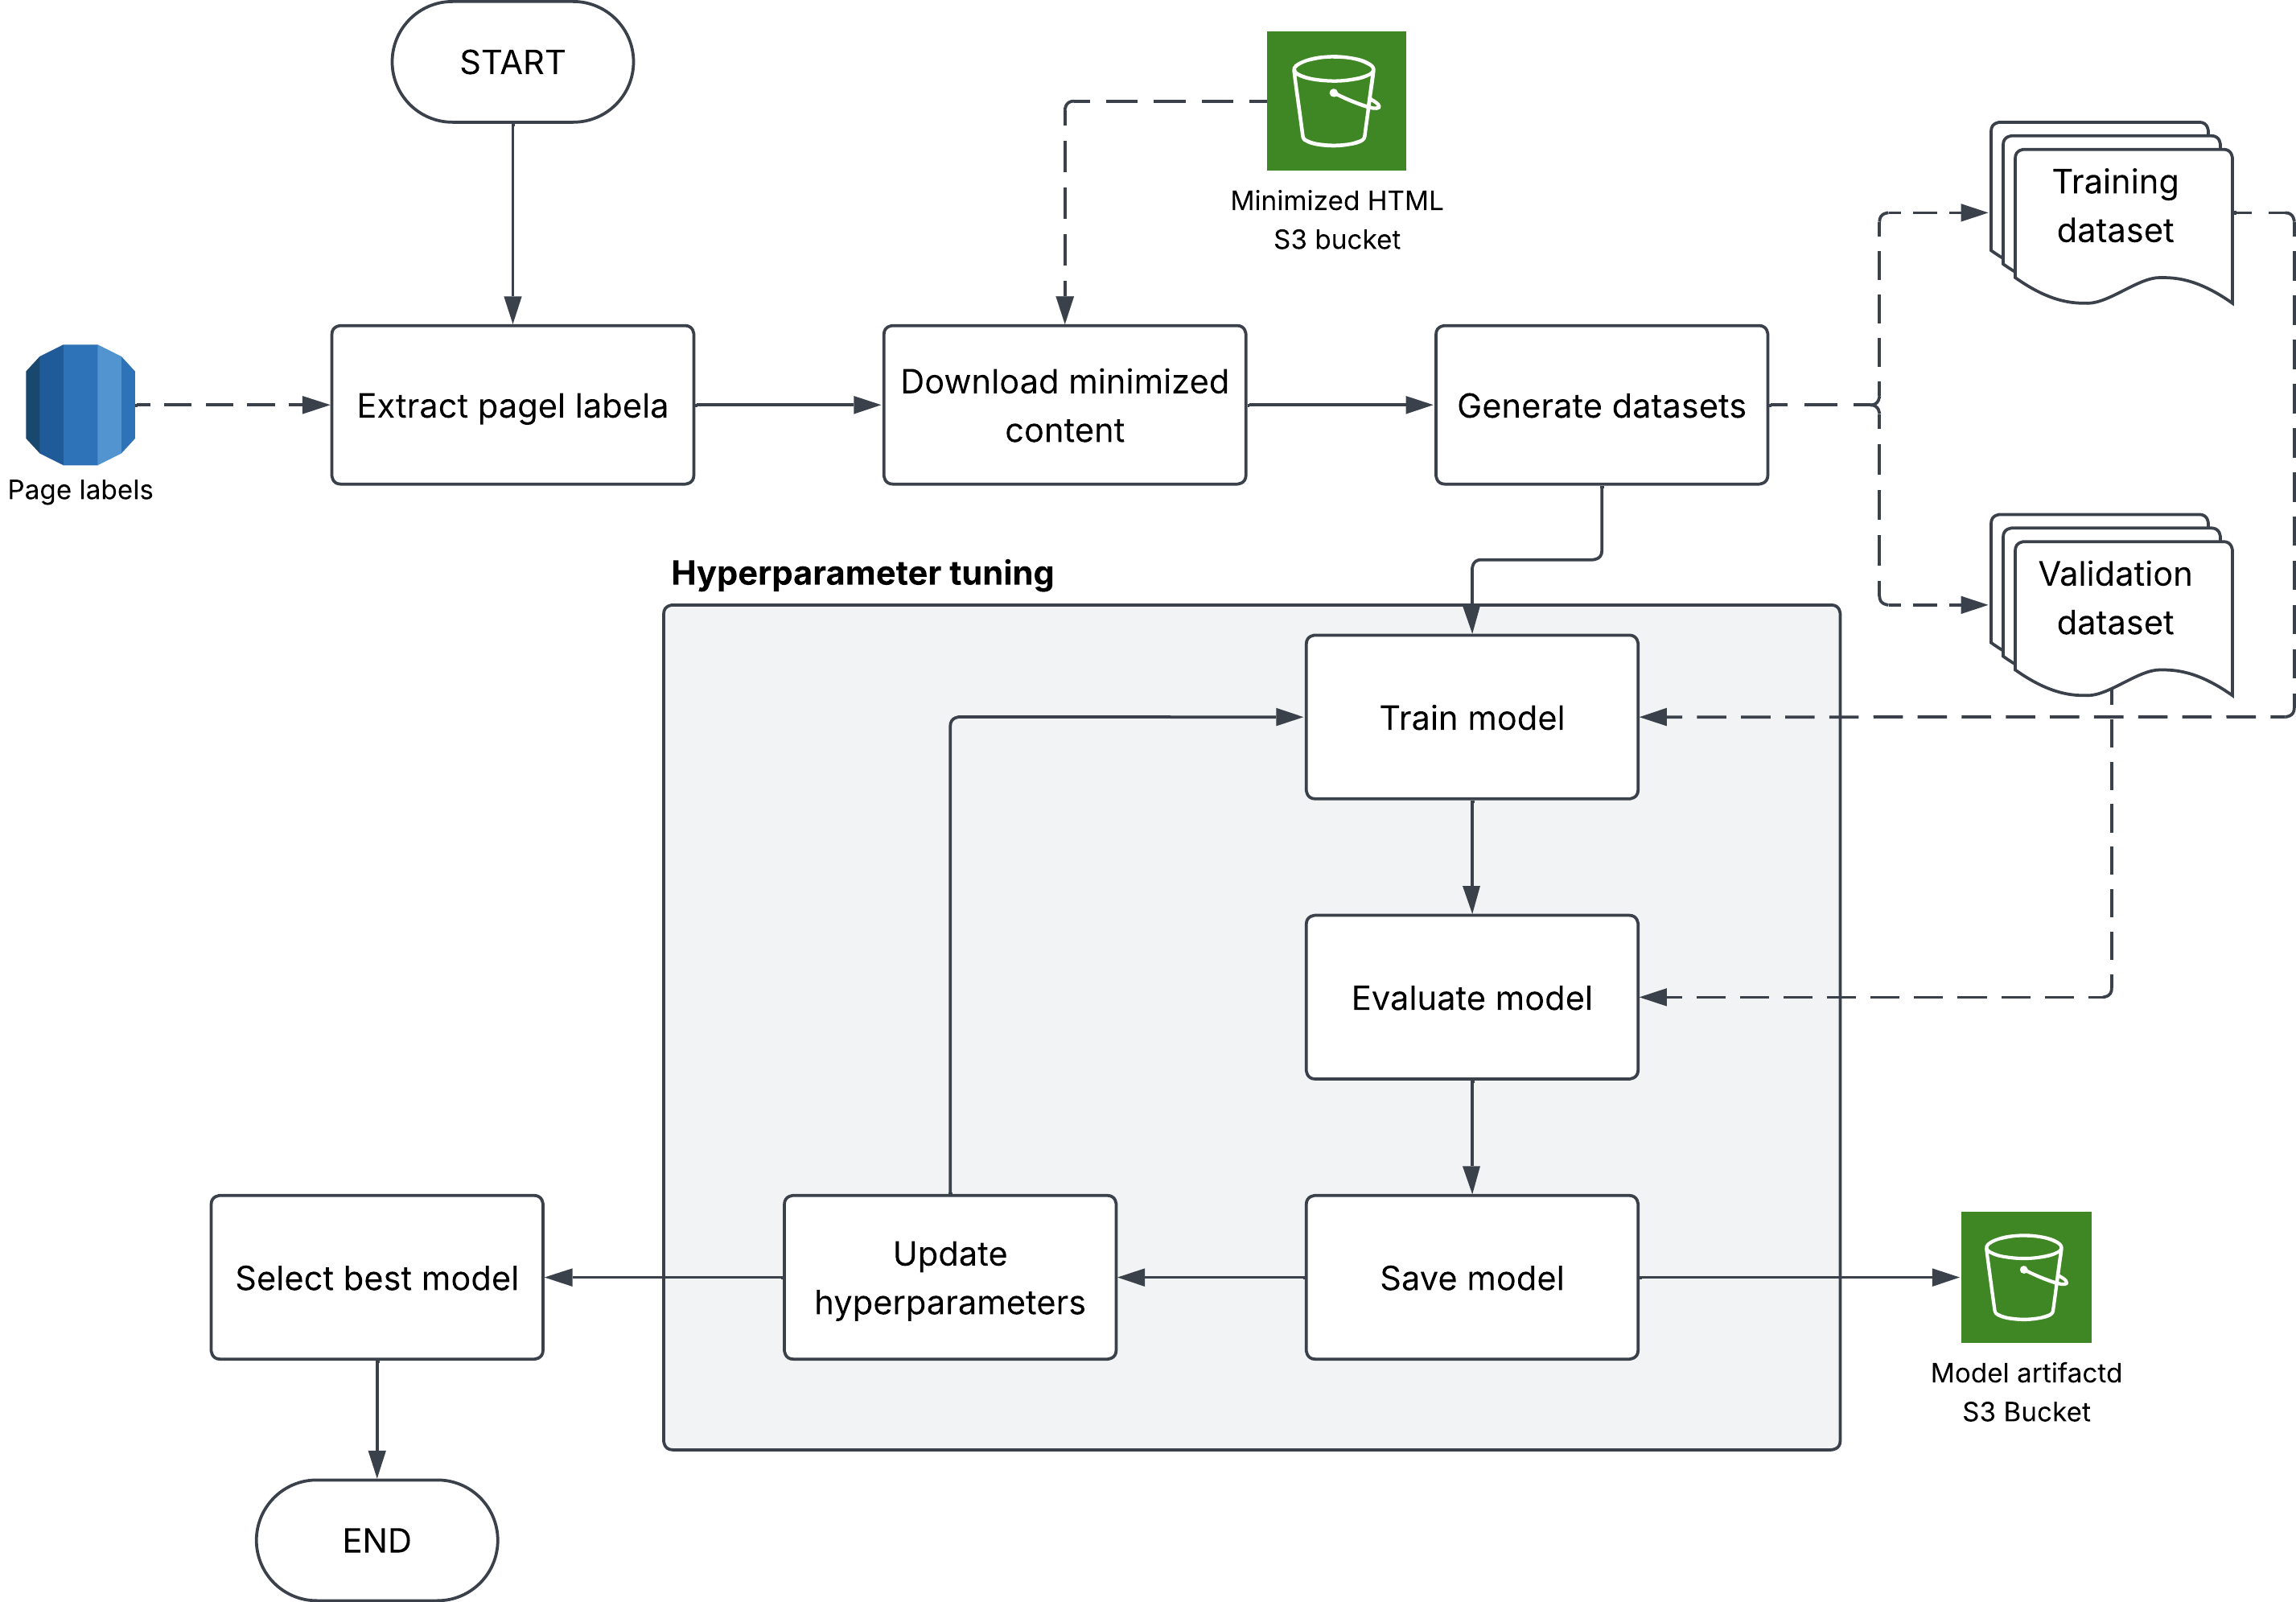
\includegraphics[width=1\textwidth]{images/page_classification_model_training}
    \caption{Overview of the page classification model training phase.}
    \label{fig:page_classifier_training_phase}
\end{figure}

\subsection{Model Evaluation and Selection}\label{subsec:page_classifier_model_evaluation}

The results of the best performing model for each approach are summarized in Table~\ref{tab:page_classifier_results}.
While the F1-score is the primary metric for evaluating the model's performance, other factors such as training and inference speed, as well as cost, were also considered when selecting the best model for deployment.

\begin{table}[h]
    \centering
    \small
    \renewcommand{\arraystretch}{1.4}
    \begin{tabularx}{\textwidth}{p{4cm} p{1.8cm} X X}
        \toprule
        \textbf{Technique} & \textbf{F1 Score} & \textbf{Pros} & \textbf{Cons} \\
        \midrule
        TF-IDF with Random Forest Regressor &
        0.930 &
        \begin{minipage}[t]{\linewidth}\raggedright \textbullet{} Very fast training and inference (\textasciitilde{}3 mins for 20,000 classifications)\par \textbullet{} Extremely cheap inference (\textasciitilde{}\$0.03 for 20,000 classifications)\end{minipage} &
        \begin{minipage}[t]{\linewidth}\raggedright \textbullet{} Low performance\end{minipage} \\
        \midrule
        BERT Embeddings with Neural Network &
        0.963 &
        \begin{minipage}[t]{\linewidth}\raggedright \textbullet{} Decent training and inference speed (\textasciitilde{}6 mins for 20,000 classifications)\par \textbullet{} Somewhat cheap inference (\textasciitilde{}\$0.22 for 20,000 classifications)\end{minipage} &
        \begin{minipage}[t]{\linewidth}\raggedright \textbullet{} Requires a GPU-accelerated machine\end{minipage} \\
        \midrule
        MarkupLM classification &
        0.989 &
        \begin{minipage}[t]{\linewidth}\raggedright \textbullet{} Extremely accurate\end{minipage} &
        \begin{minipage}[t]{\linewidth}\raggedright \textbullet{} Requires a GPU-accelerated machine\par \textbullet{} Slow training and inference (\textasciitilde{}13 mins for 20,000 classifications)\par \textbullet{} Expensive (\textasciitilde{}\$0.40 for 20,000 classifications)\end{minipage} \\
        \bottomrule
    \end{tabularx}
    \caption{Comparison of page classification approaches}
    \label{tab:page_classifier_results}
\end{table}

Based on the results in Table~\ref{tab:page_classifier_results}, the BERT embeddings with a neural network classifier approach was selected for deployment in the inference phase, as it provides a good balance between accuracy, speed, and cost.

\subsection{Inference Phase}\label{subsec:page_classifier_inference_phase}

The inference phase involves using the best performing model from the training phase to classify new crawled pages as product pages or non-product pages.
This is implemented as a scheduled batch job that runs once a day.
In each run, the following steps are performed:
\begin{enumerate}
    \item Fetch the list of recently crawled pages that have not yet been classified from the database.
    \item For each page, fetch the minimized HTML content from the S3 bucket.
    \item For each page, generate BERT embeddings from the minimized HTML content.
    \item For each page, use the trained neural network classifier to classify the page as a product page or a non-product page.
    \item Store the classification results in the database, along with the relevant metadata, such as the page URL and the timestamp of the classification.
\end{enumerate}

This pipeline is implemented using AWS Step Functions, which orchestrates the different steps of the pipeline and ensures that they are executed in the correct order.
It also provides error handling and retry mechanisms to ensure that the pipeline can recover from failures (especially due to unavailability of compute resources in AWS) and continue processing the remaining stages.
Figure ~\ref{fig:page_classifier_inference_phase} illustrates the overall architecture of the page classification inference phase.

\begin{figure}[h]
    \centering
    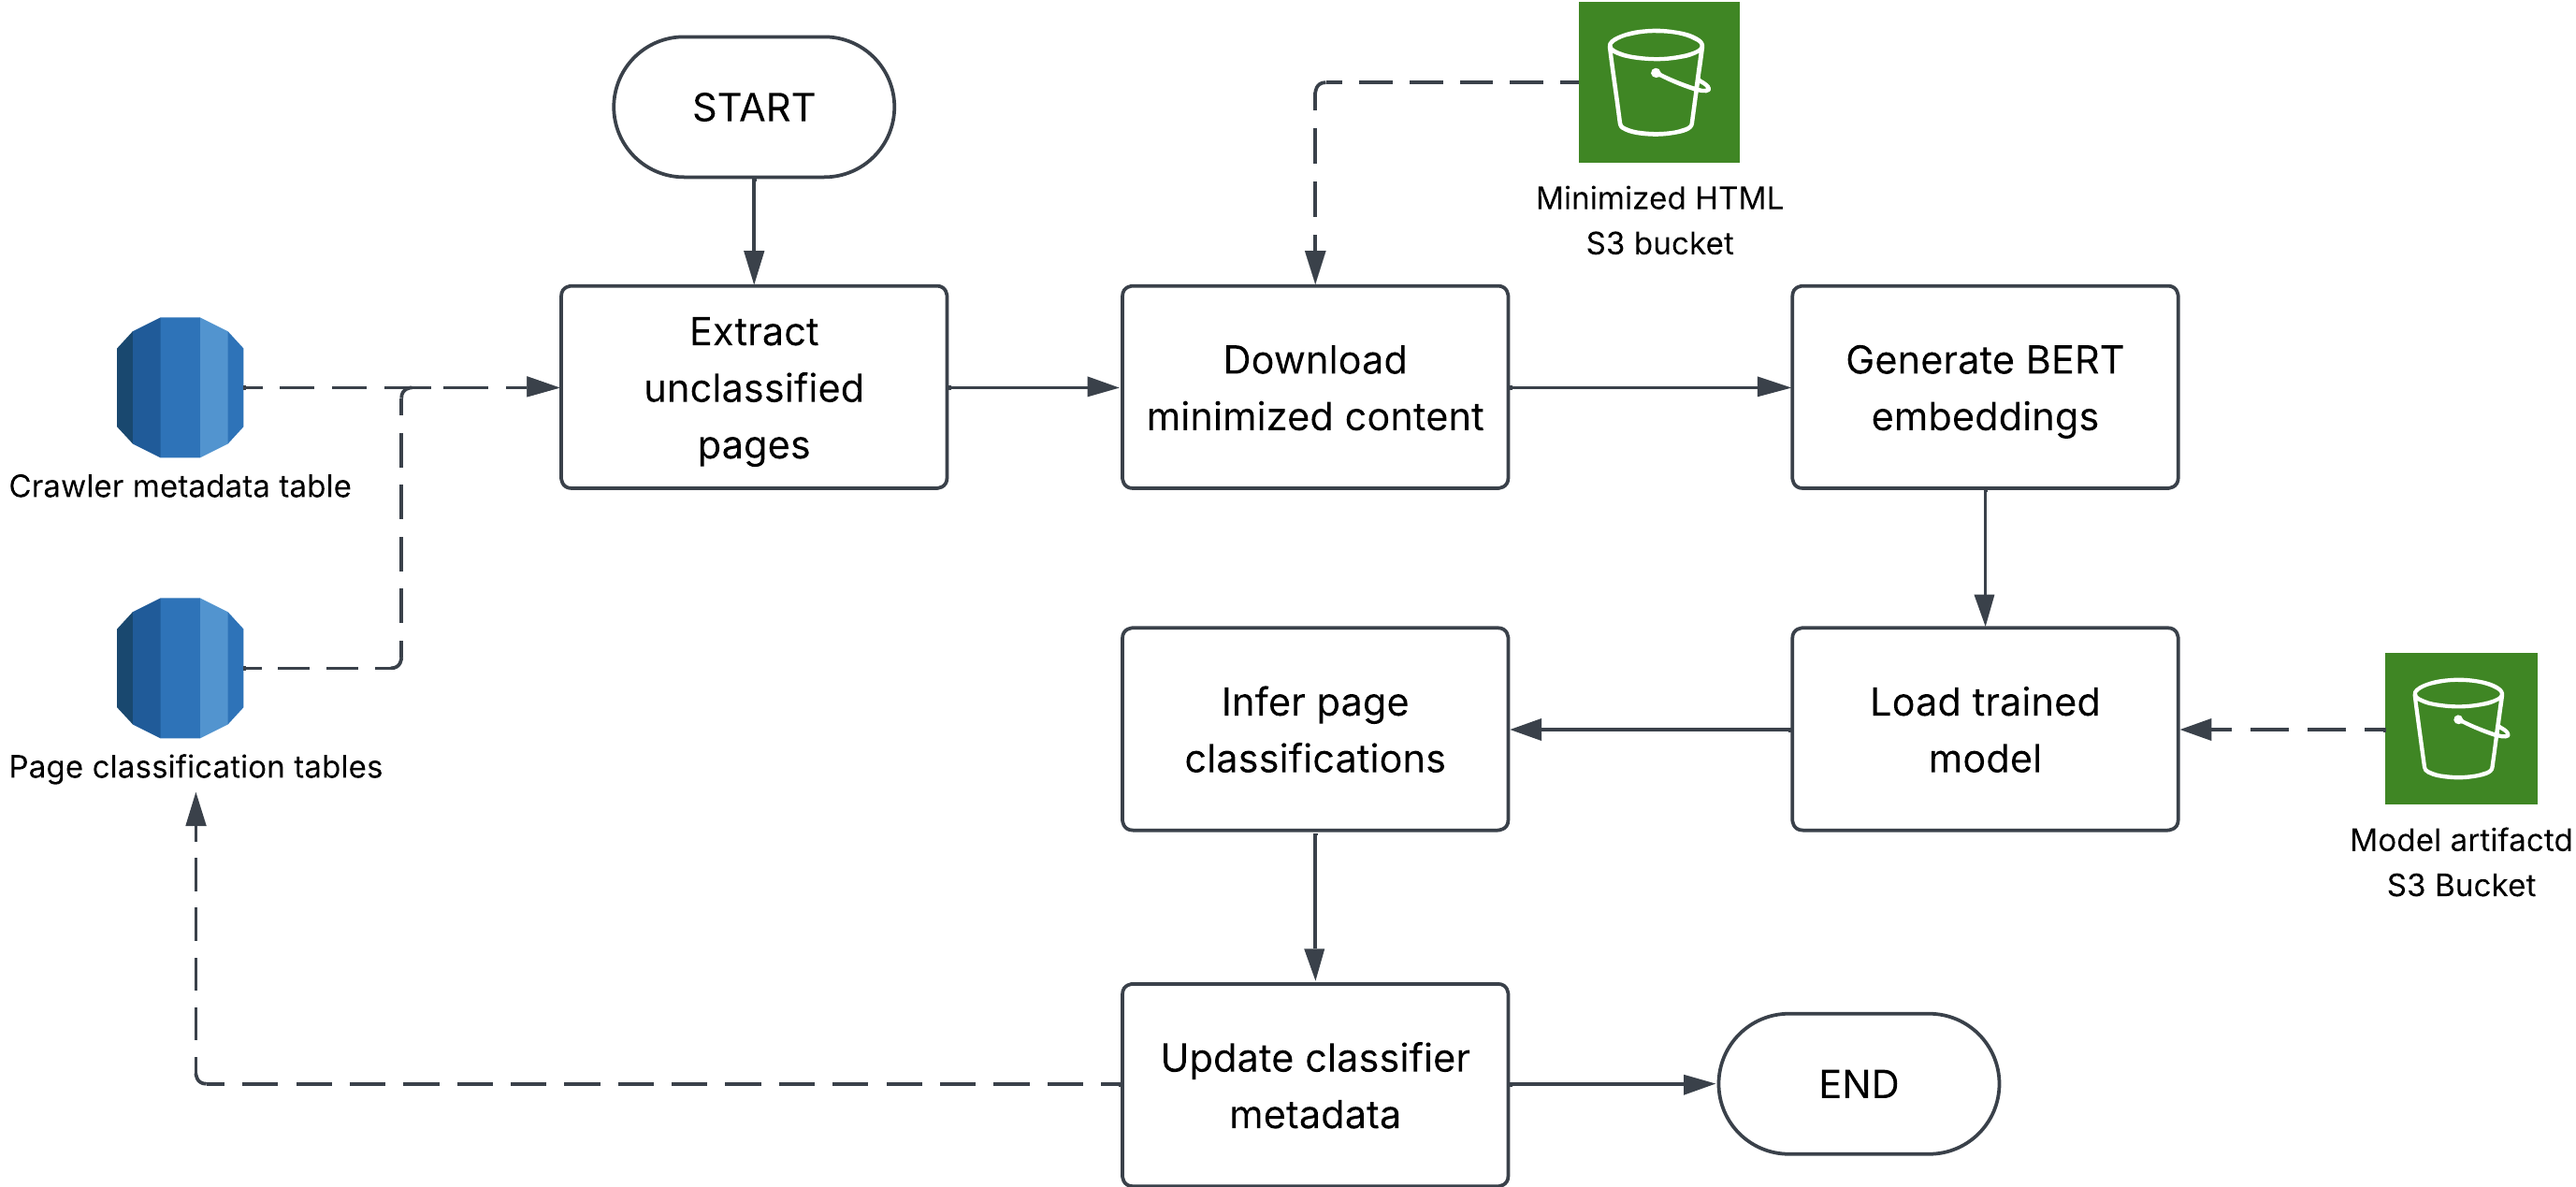
\includegraphics[width=1\textwidth]{images/page_classification_inference}
    \caption{Overview of the page classification inference phase.}
    \label{fig:page_classifier_inference_phase}
\end{figure}

\subsection{Page Classifier Architecture}\label{subsec:page_classifier_architecture}

The page classifier architecture is designed to be scalable and efficient, allowing for the processing of large volumes of crawled pages in a timely manner.
Figure~\ref{fig:page_classifier_architecture} illustrates the overall architecture of the page classifier module, which includes the different components involved in the training and inference phases, as well as the interactions with the database and S3 buckets.

\begin{figure}[h]
    \centering
    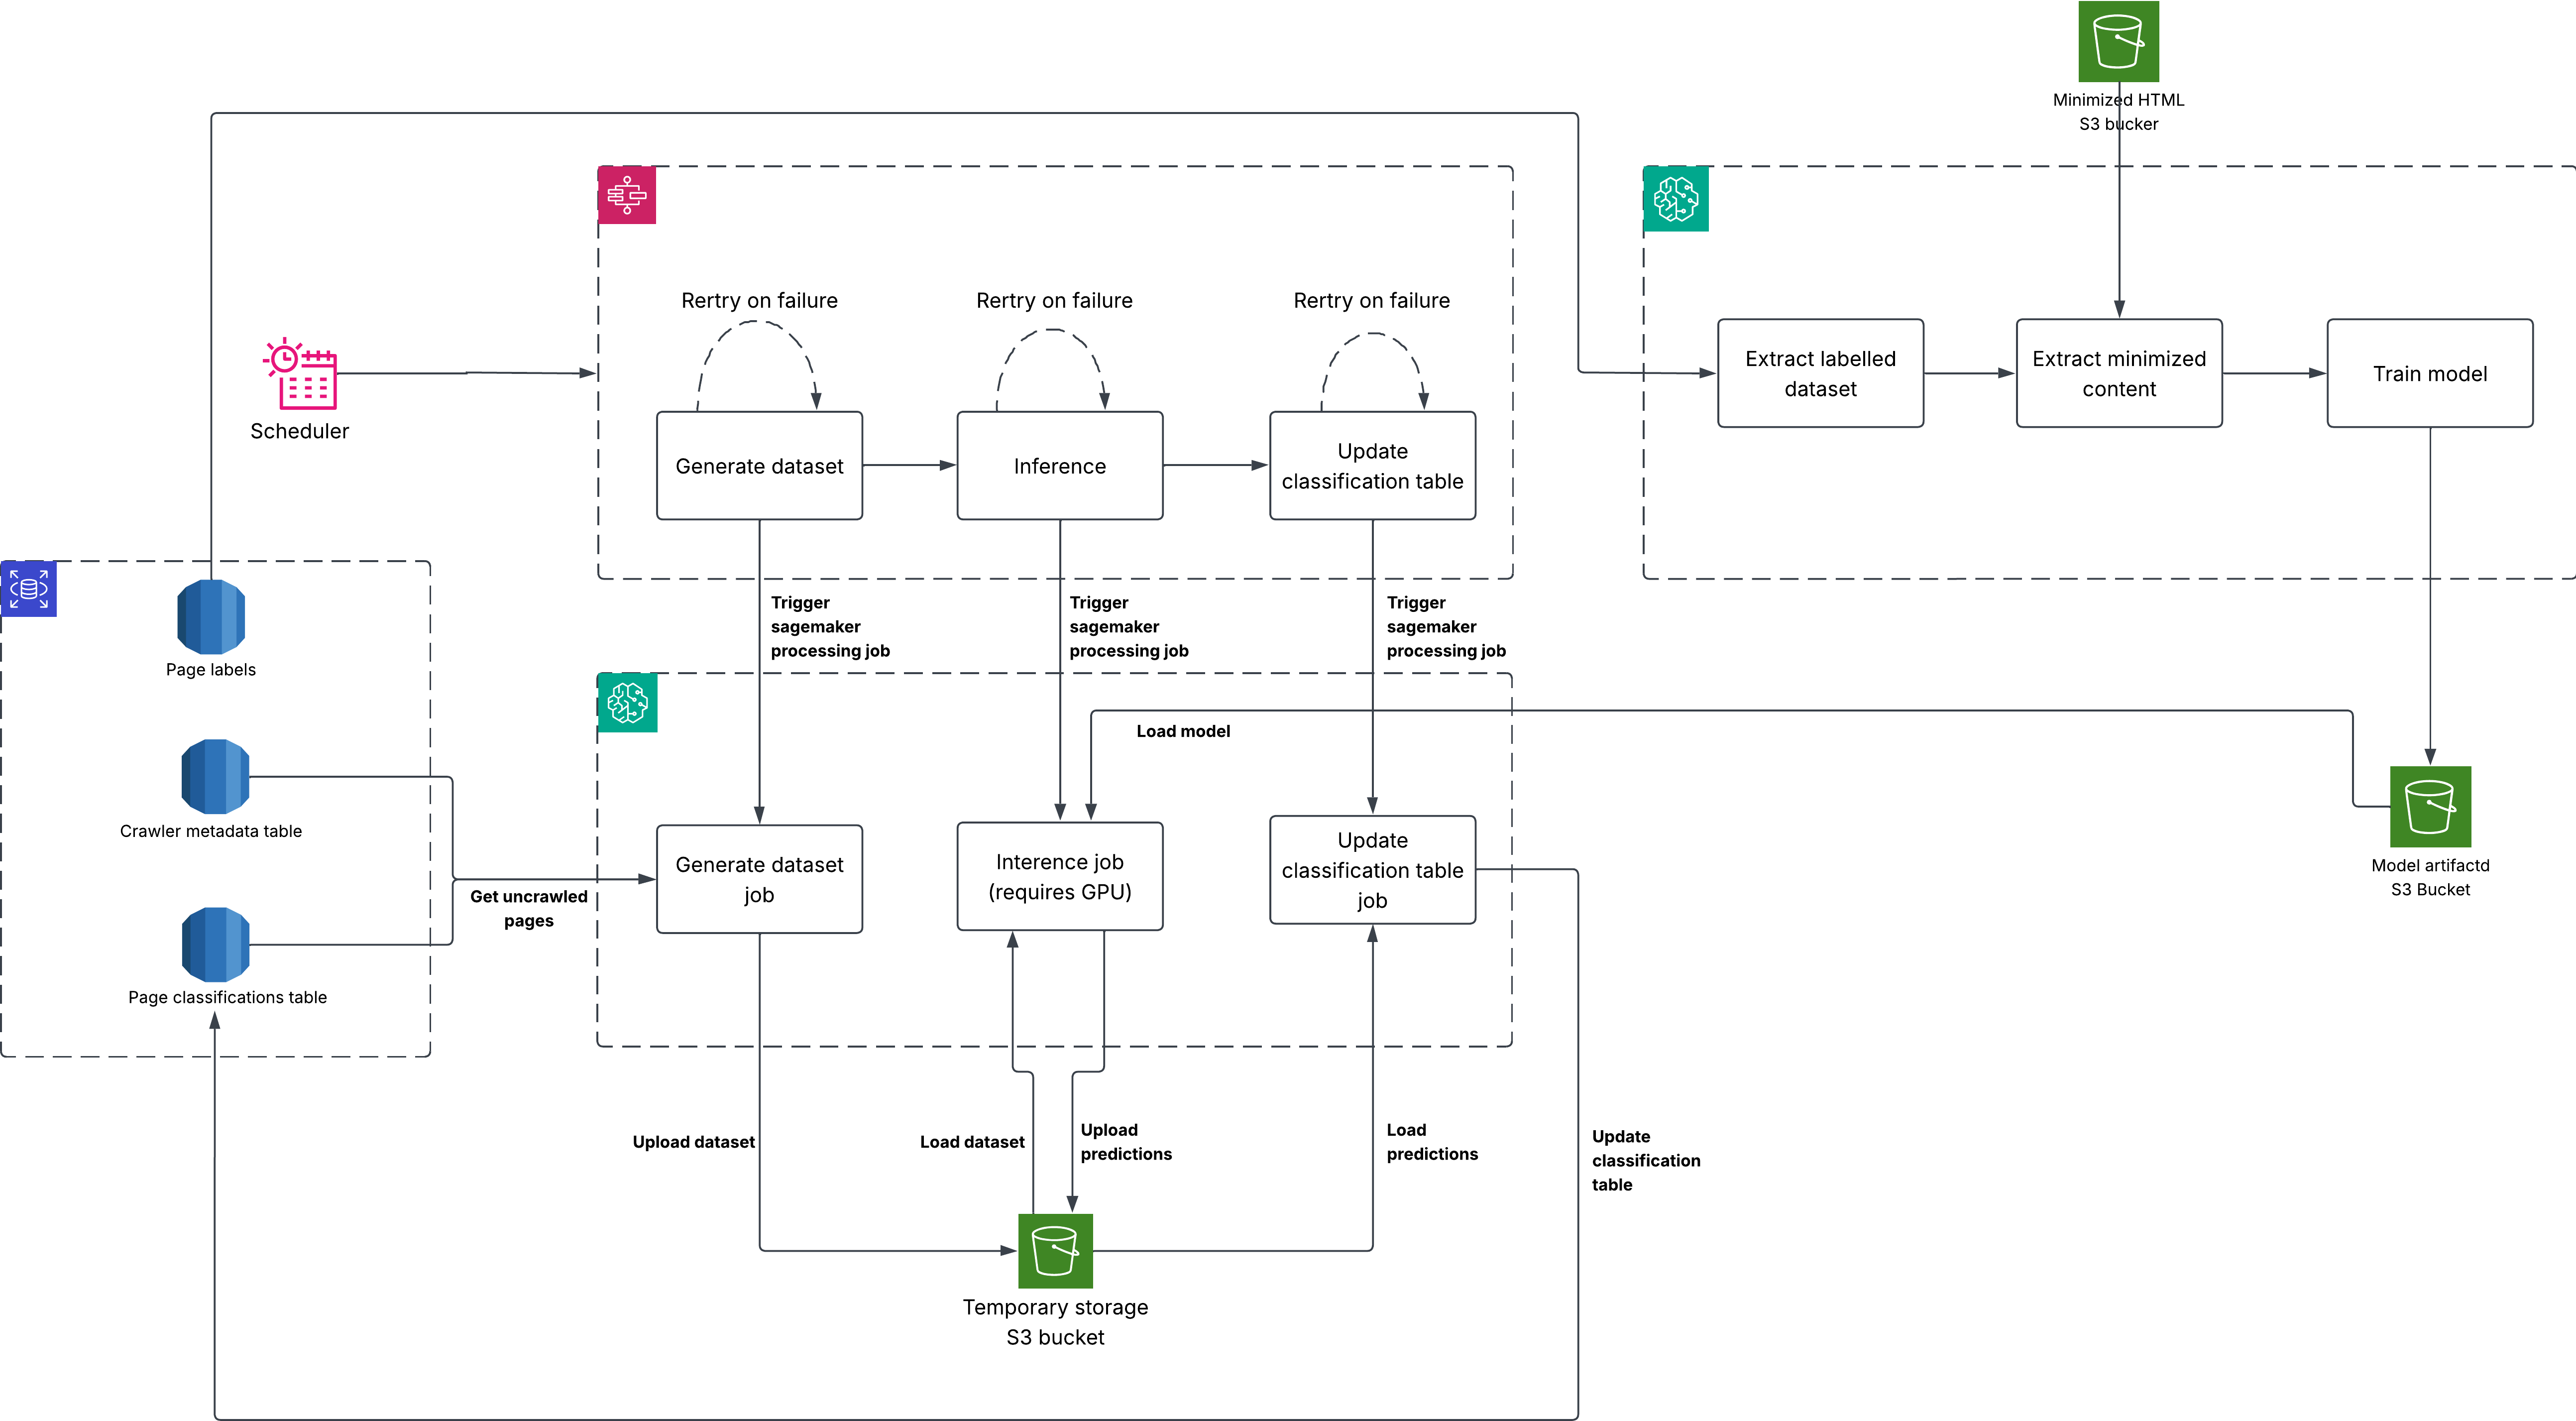
\includegraphics[width=1\textwidth]{images/page_classification_architecture}
    \caption{Overview of the page classifier architecture.}
    \label{fig:page_classifier_architecture}
\end{figure}